\chapter{Results}
\index{Results@\emph{Results}}%


\section{word and song prosodic prominence}


\subsection{Duration of Vowels}

%
\begin{figure}[htb]
\begin{center}
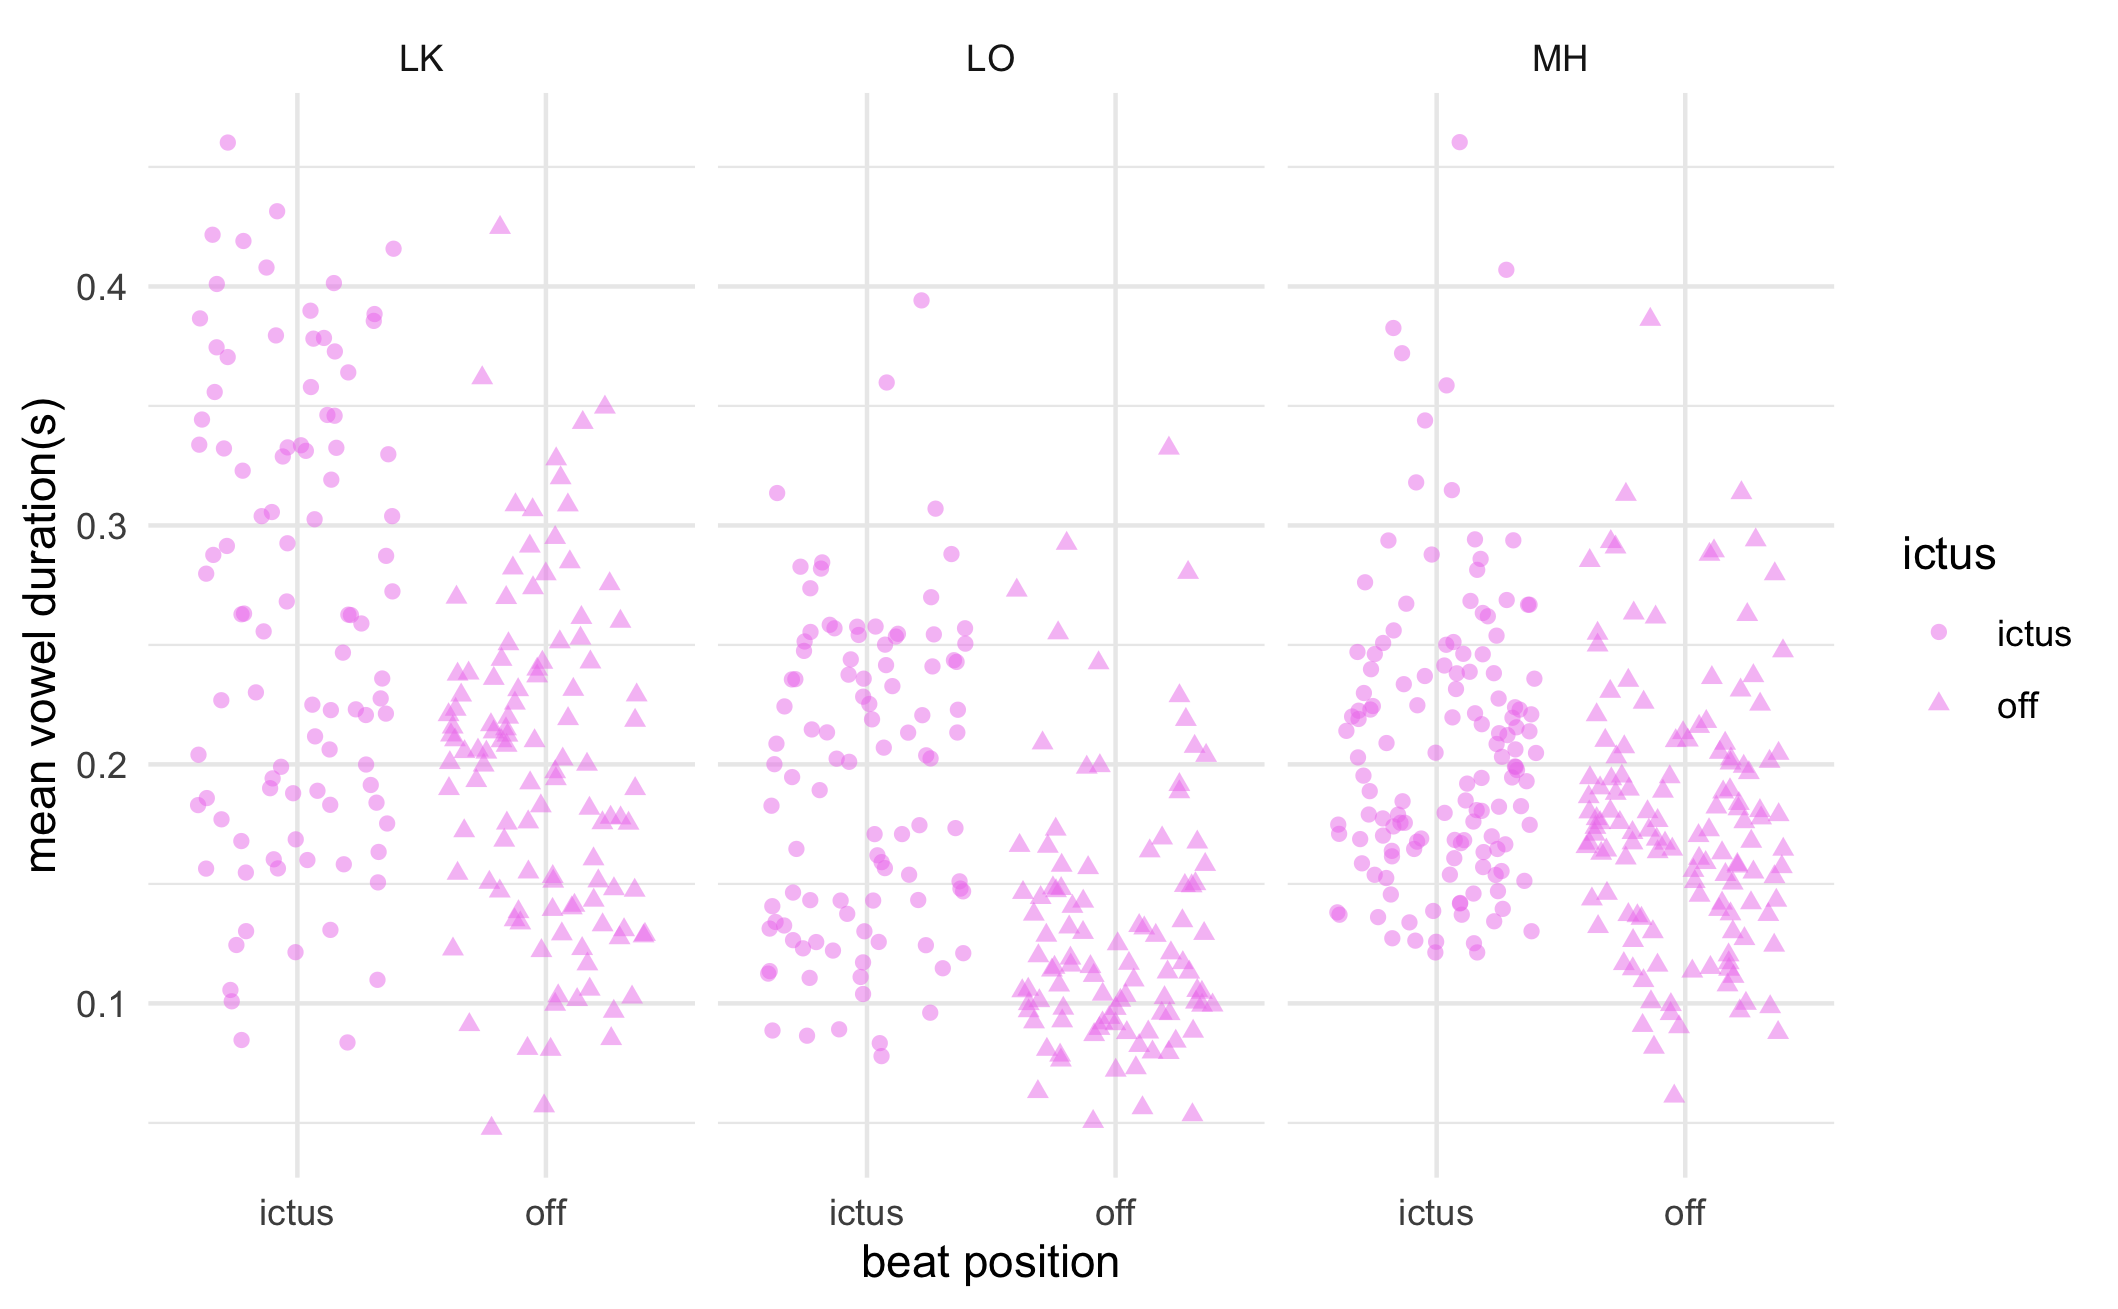
\includegraphics[width=\textwidth]{/Users/sarah/Git/regilaul_project/manuscript/results/perf_ick_dur.png}

\caption{}
\label{songick}
\end{center}
\end{figure}
%In \ref{songick}, vowel durations of syllable-notes that fall on the beat trend longer than those that fall off the beat. 
%
%
\begin{figure}[htb]
\begin{center}
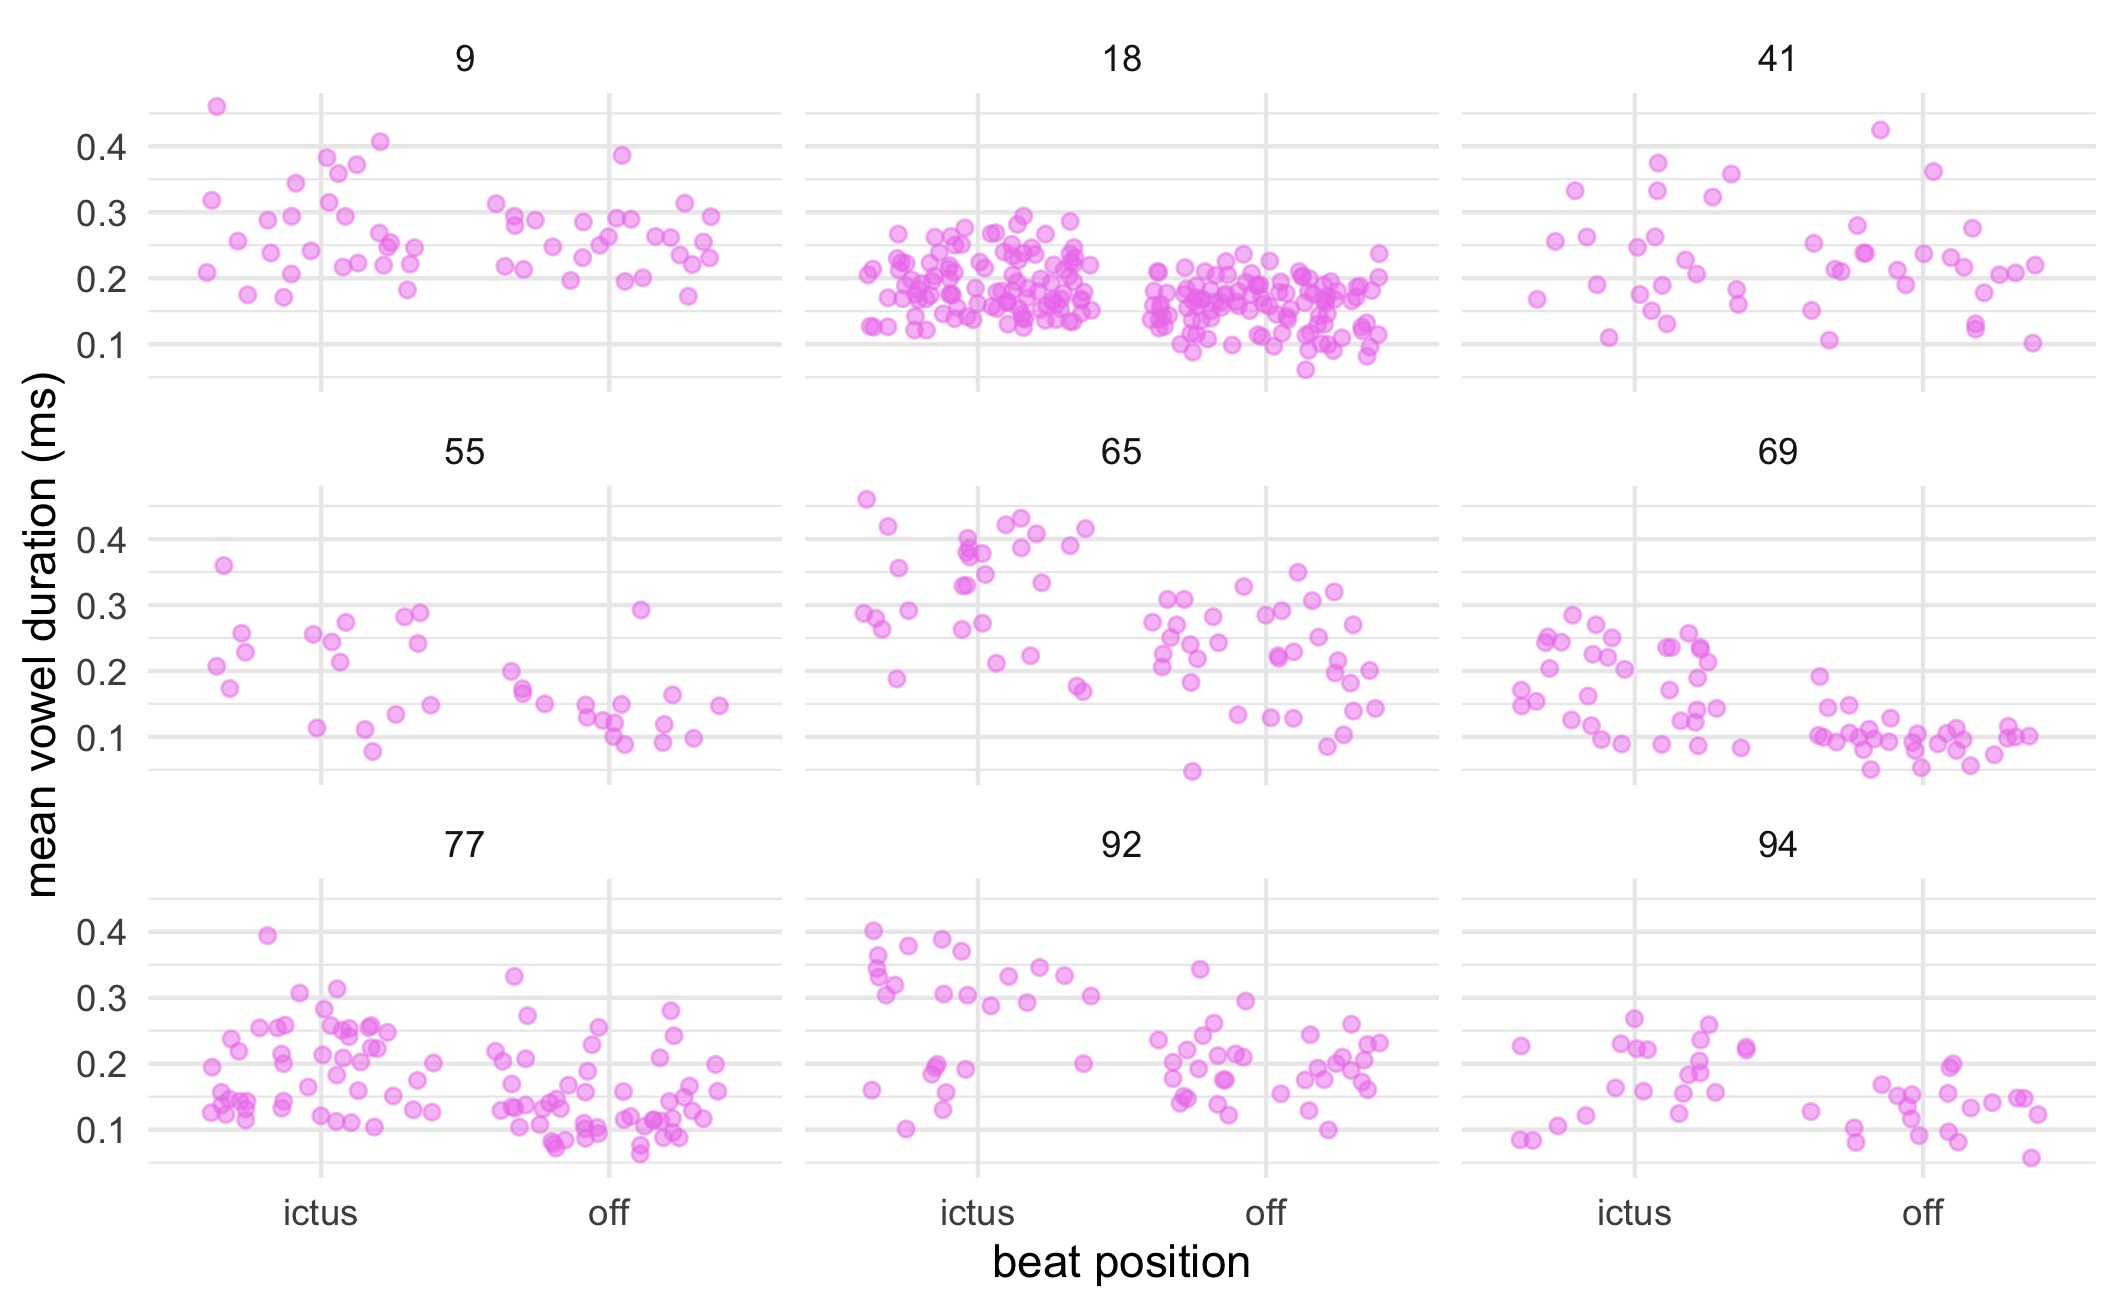
\includegraphics[width=\textwidth]{/Users/sarah/Git/regilaul_project/manuscript/results/song_icK_dur.png}

\caption{n}
\label{songstr}
\end{center}
\end{figure}

\begin{figure}[htb]
\begin{center}
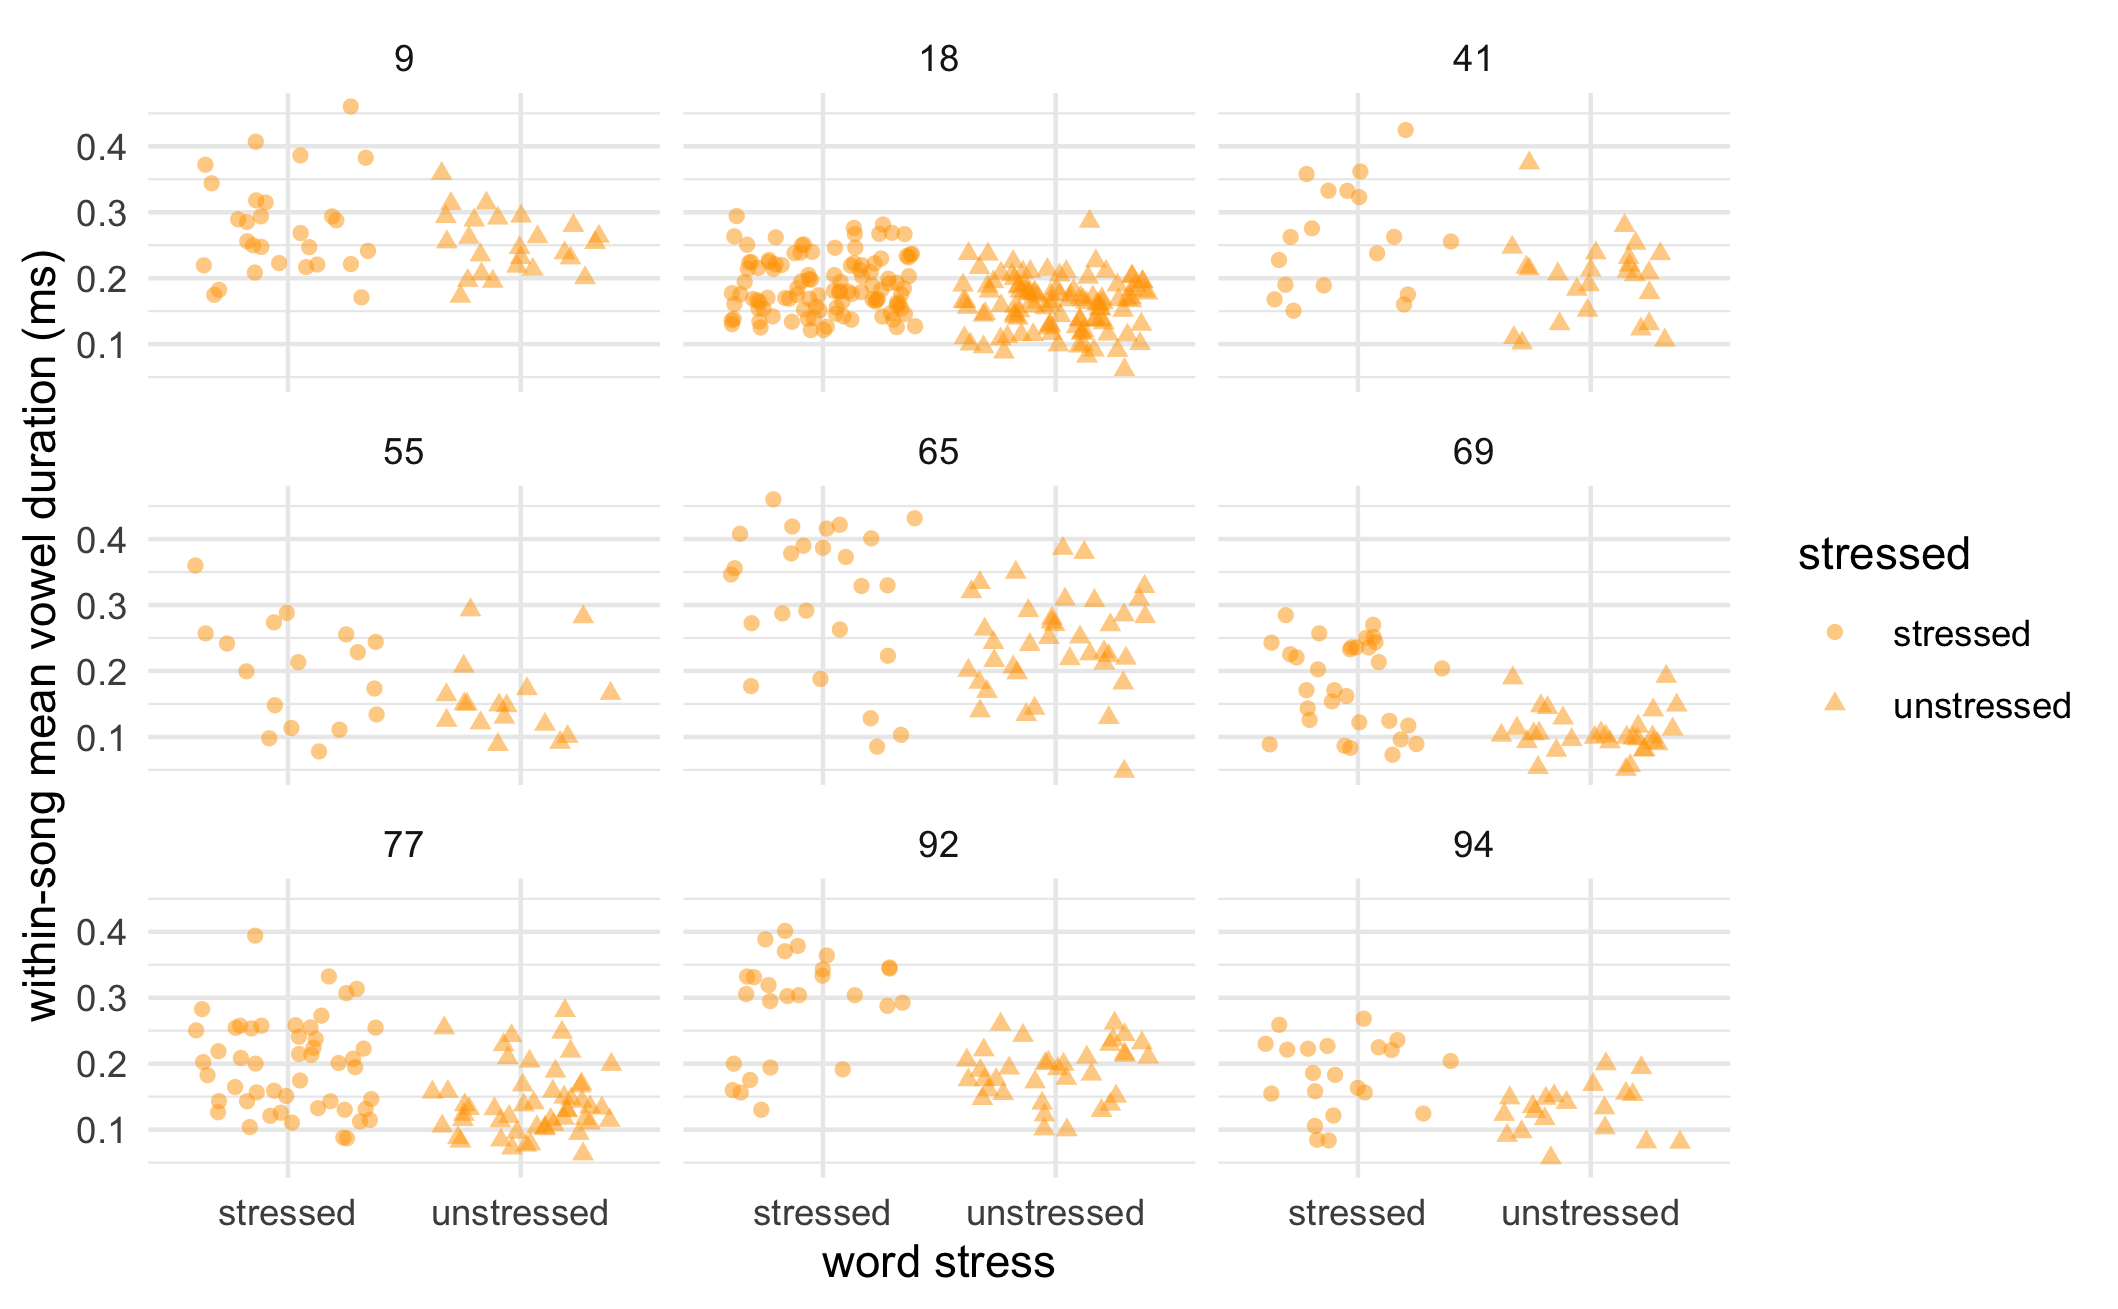
\includegraphics[width=\textwidth]{/Users/sarah/Git/regilaul_project/manuscript/results/song_str_dur.png}

\caption{within-song vowel durations and word-stress position}
\label{songstr}
\end{center}
\end{figure}

%
%with observations grouped by song \ref{songstr} shows durations of syllable nuclei in two word-stress positions: stressed and unstressed. Here it is clear that syllable-notes that are ordinarily stressed in spoken Estonian maintain the longer vowel duration even in nominally isochronous syllable-notes. 
%
%Taken together, \ref{songick} and \ref{songstr} show that within each song, vowel durations are distributed in such a way that preserves the word level duration cue of prominence (stressed vowels are longer overall) while simultaneously satisfying the expected distributions of the musical meter: syllable-notes falling on the beat have longer vowel durations than those that fall off the beat. 

\begin{figure}[htb]
\begin{center}
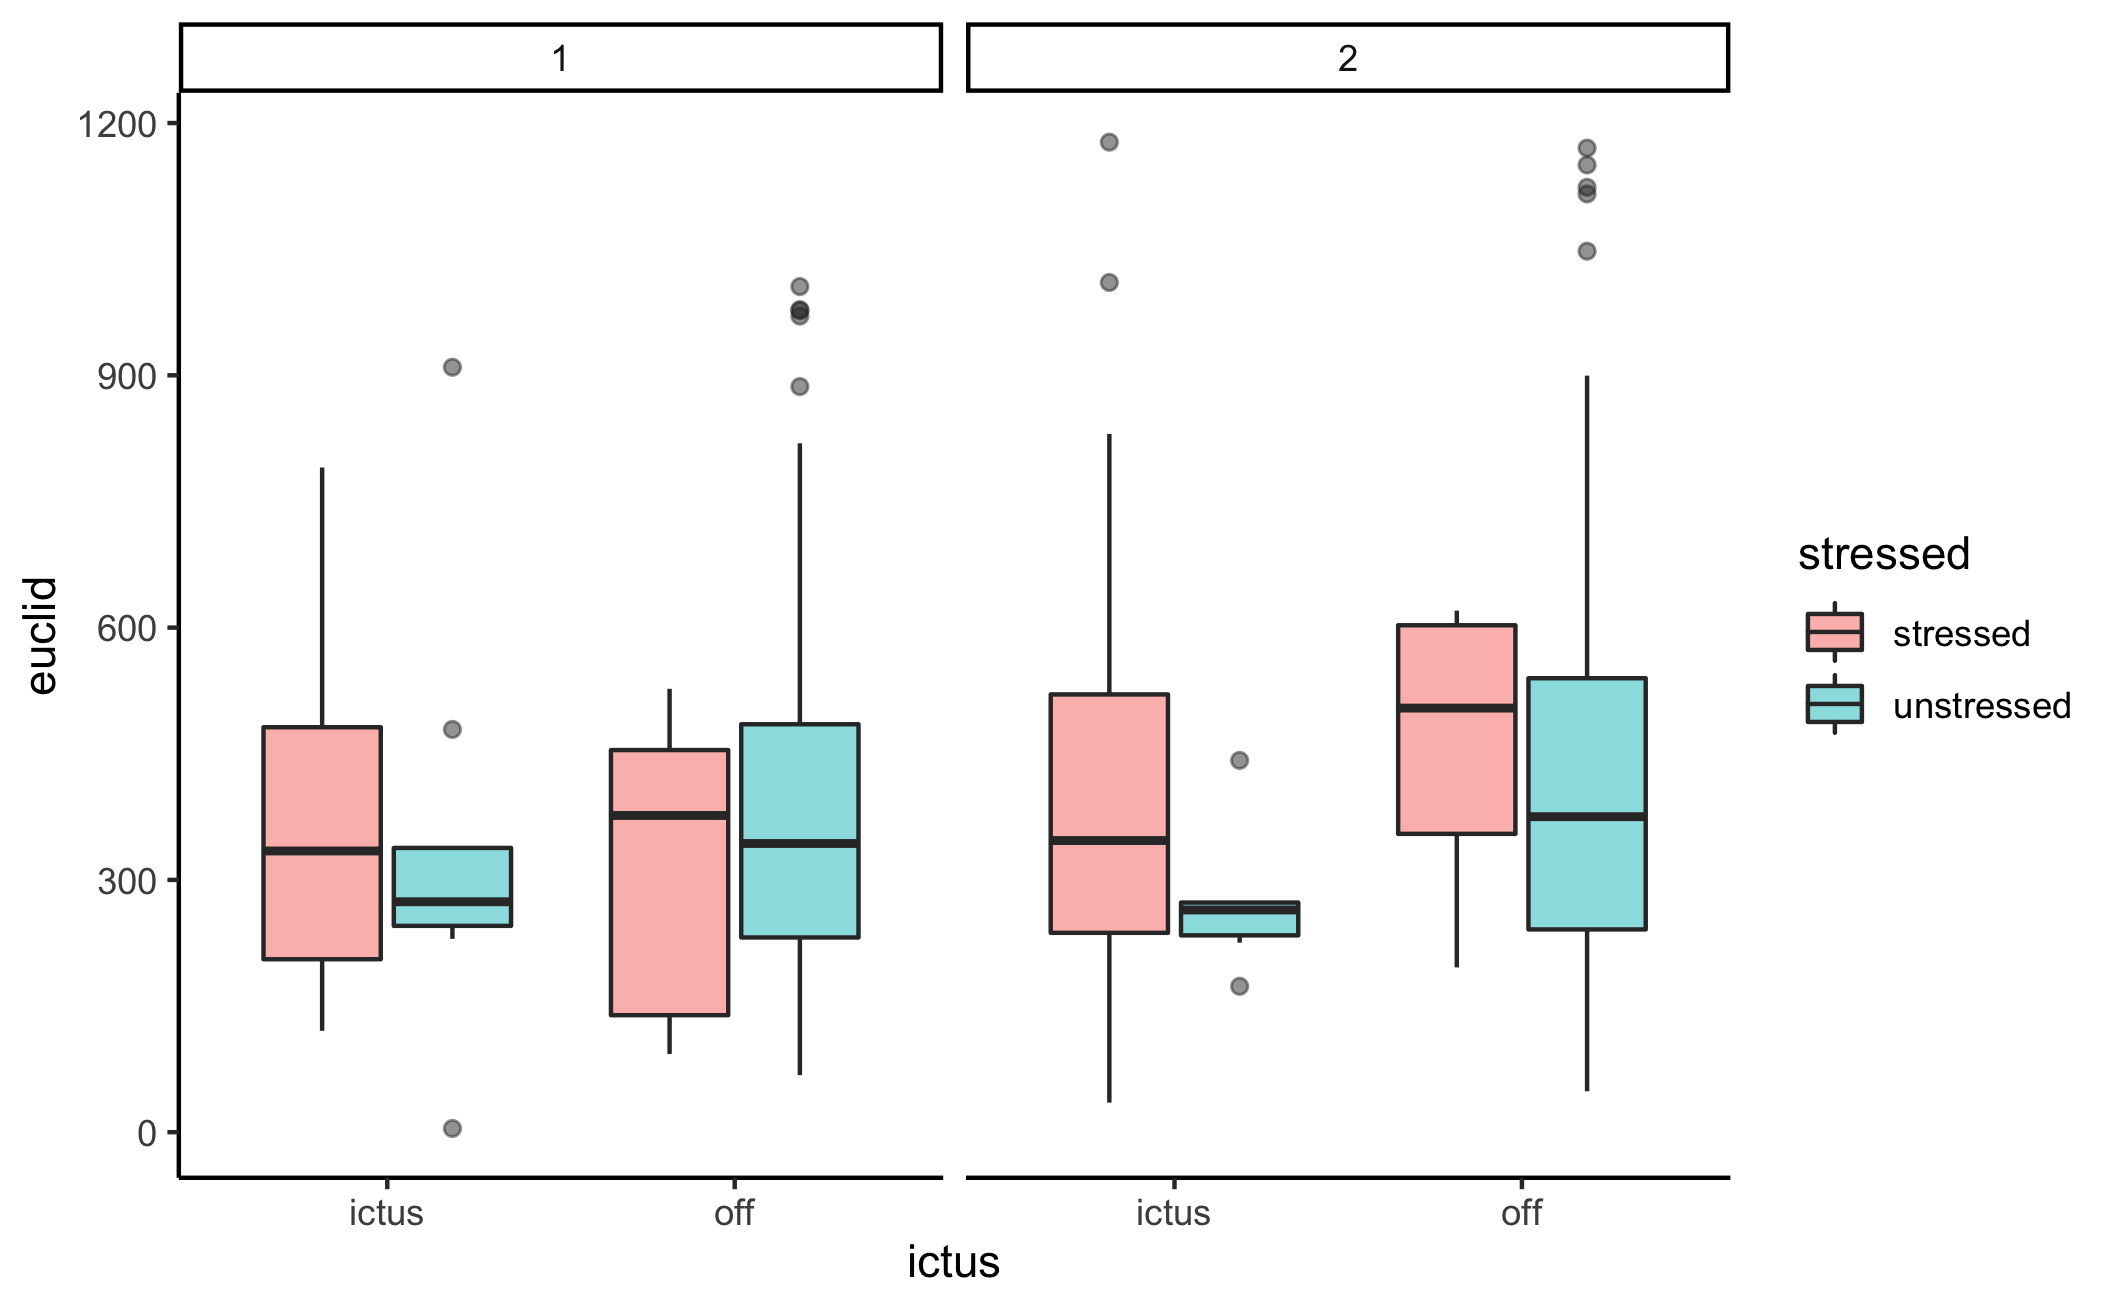
\includegraphics[width=\textwidth]{/Users/sarah/Git/regilaul_project/manuscript/results/space_strictus.png}
\caption{}
\label{}
\end{center}
\end{figure}

\begin{figure}[htbp]
\begin{center}
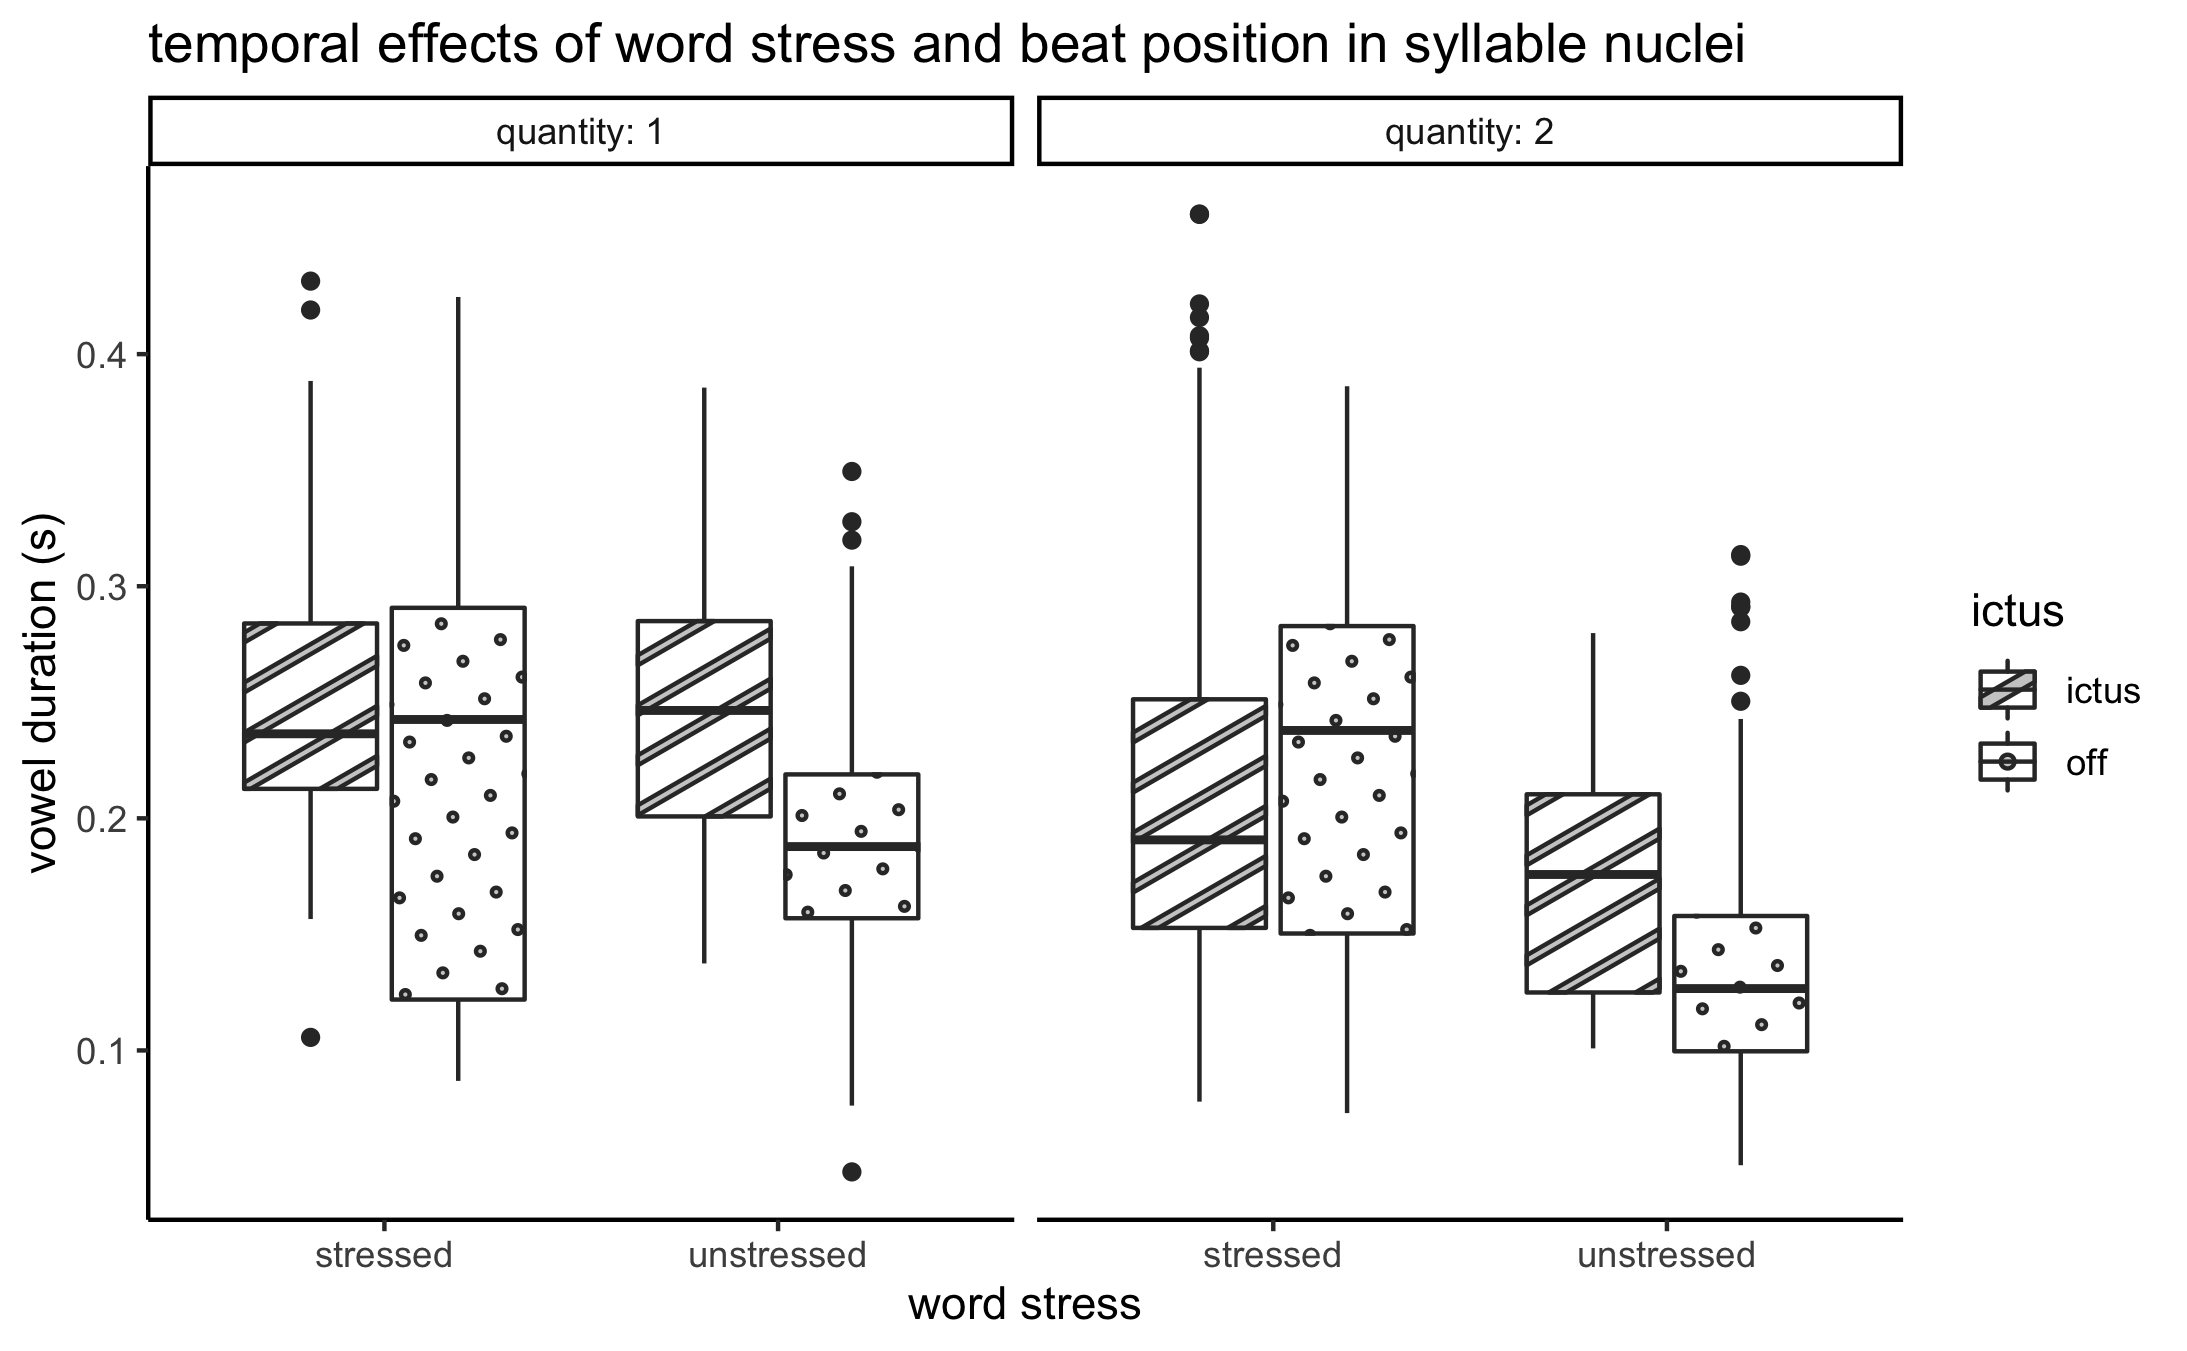
\includegraphics[width=\textwidth]{/Users/sarah/Git/regilaul_project/manuscript/results/dur_density_qfac.png}
\caption{default}
\label{default}
\end{center}
\end{figure}


\begin{figure}[htbp]
\begin{center}
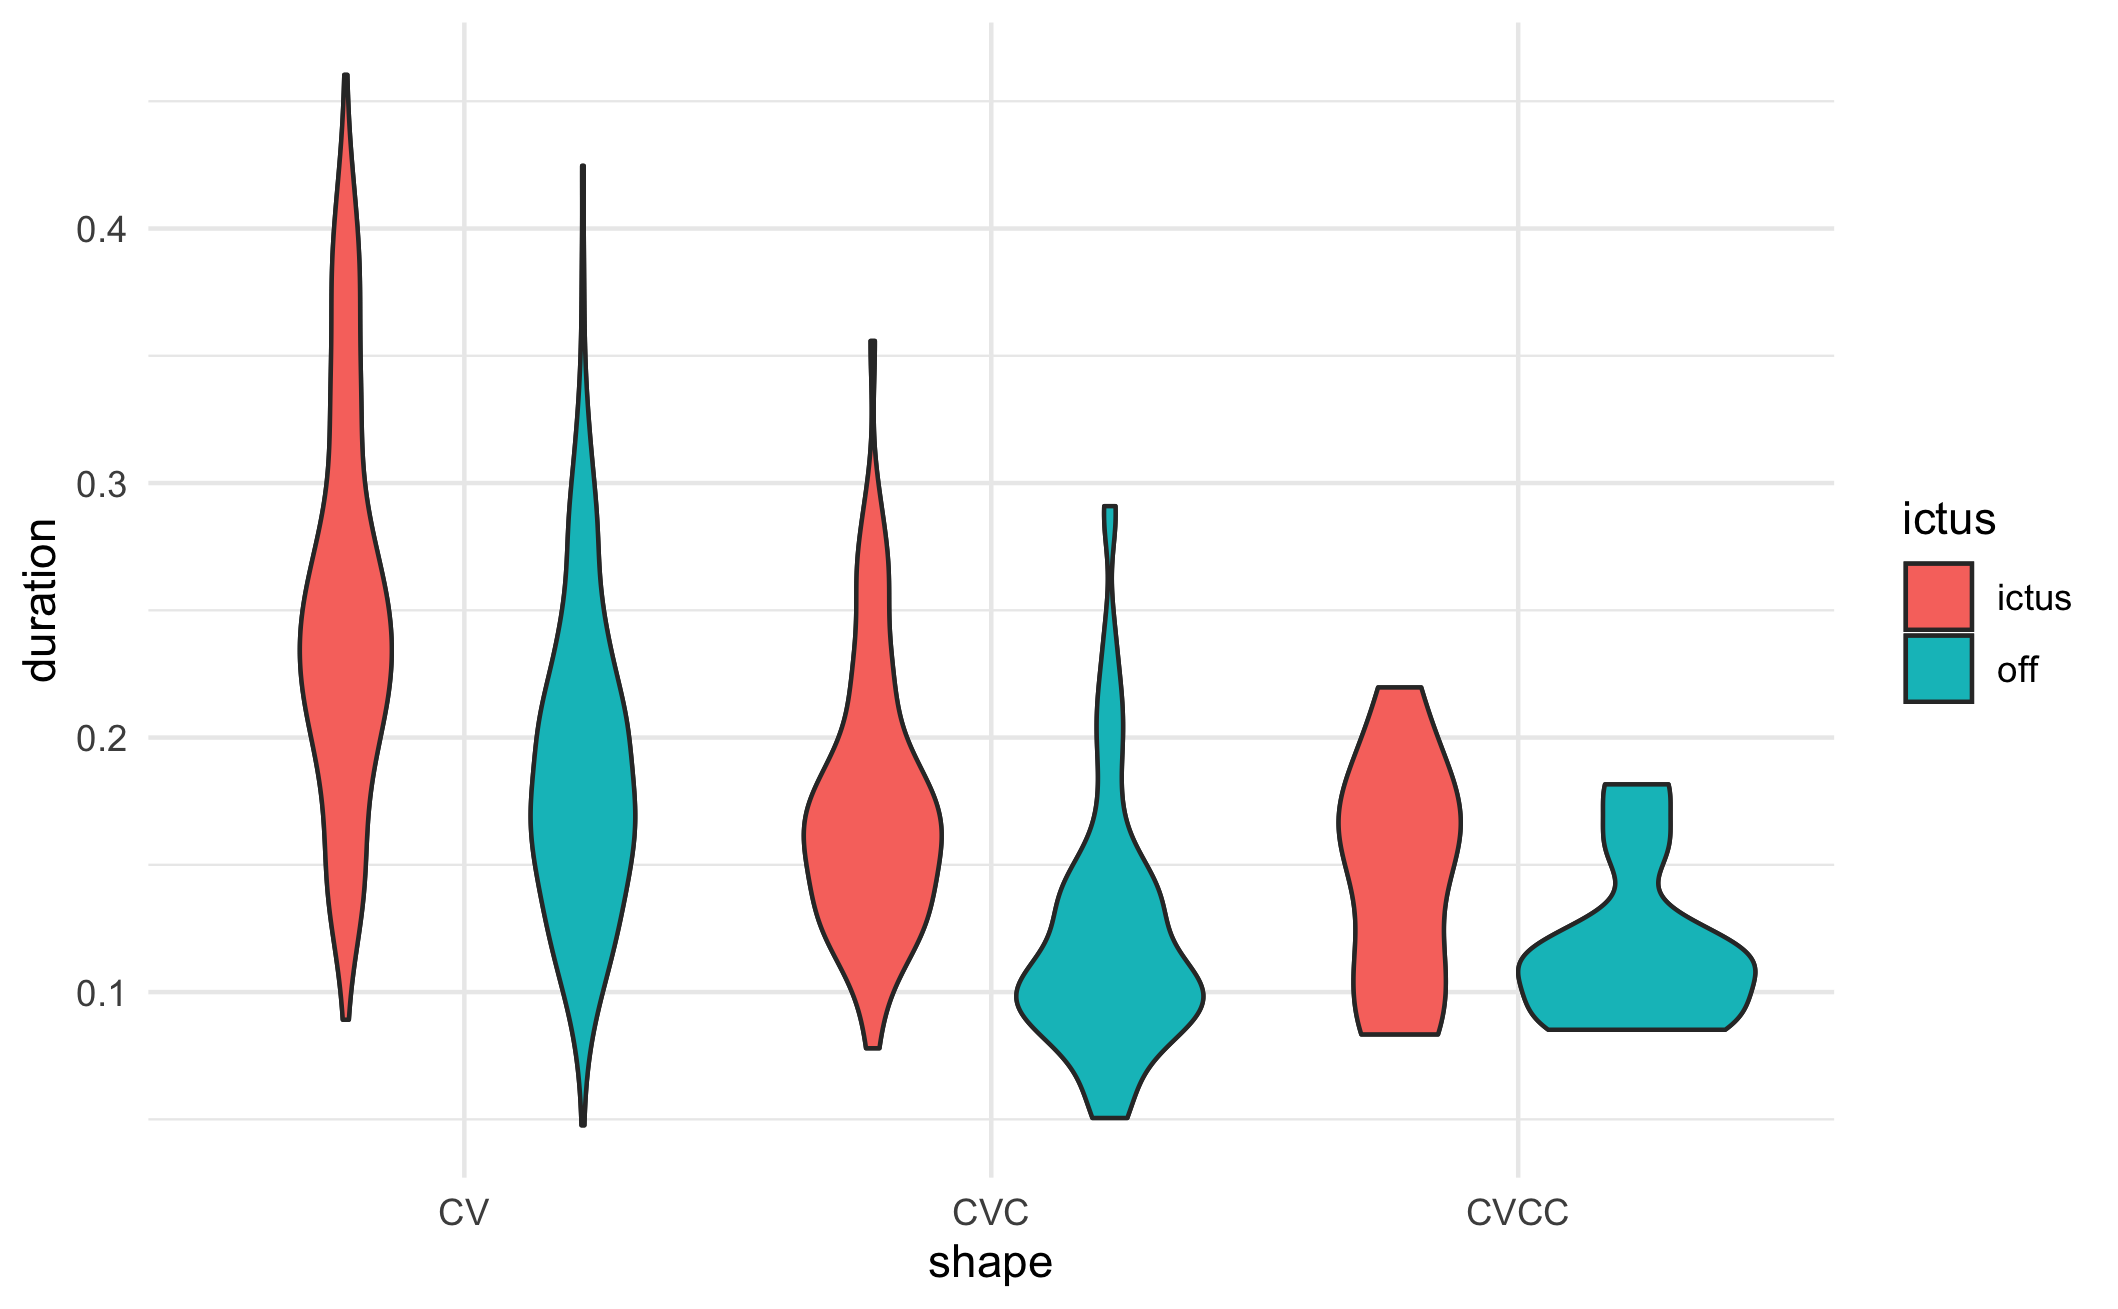
\includegraphics[width=\textwidth]{/Users/sarah/Git/regilaul_project/manuscript/results/dur_shape_ictus.png}
\caption{default}
\label{default}
\end{center}
\end{figure}

\begin{figure}[htbp]
\begin{center}
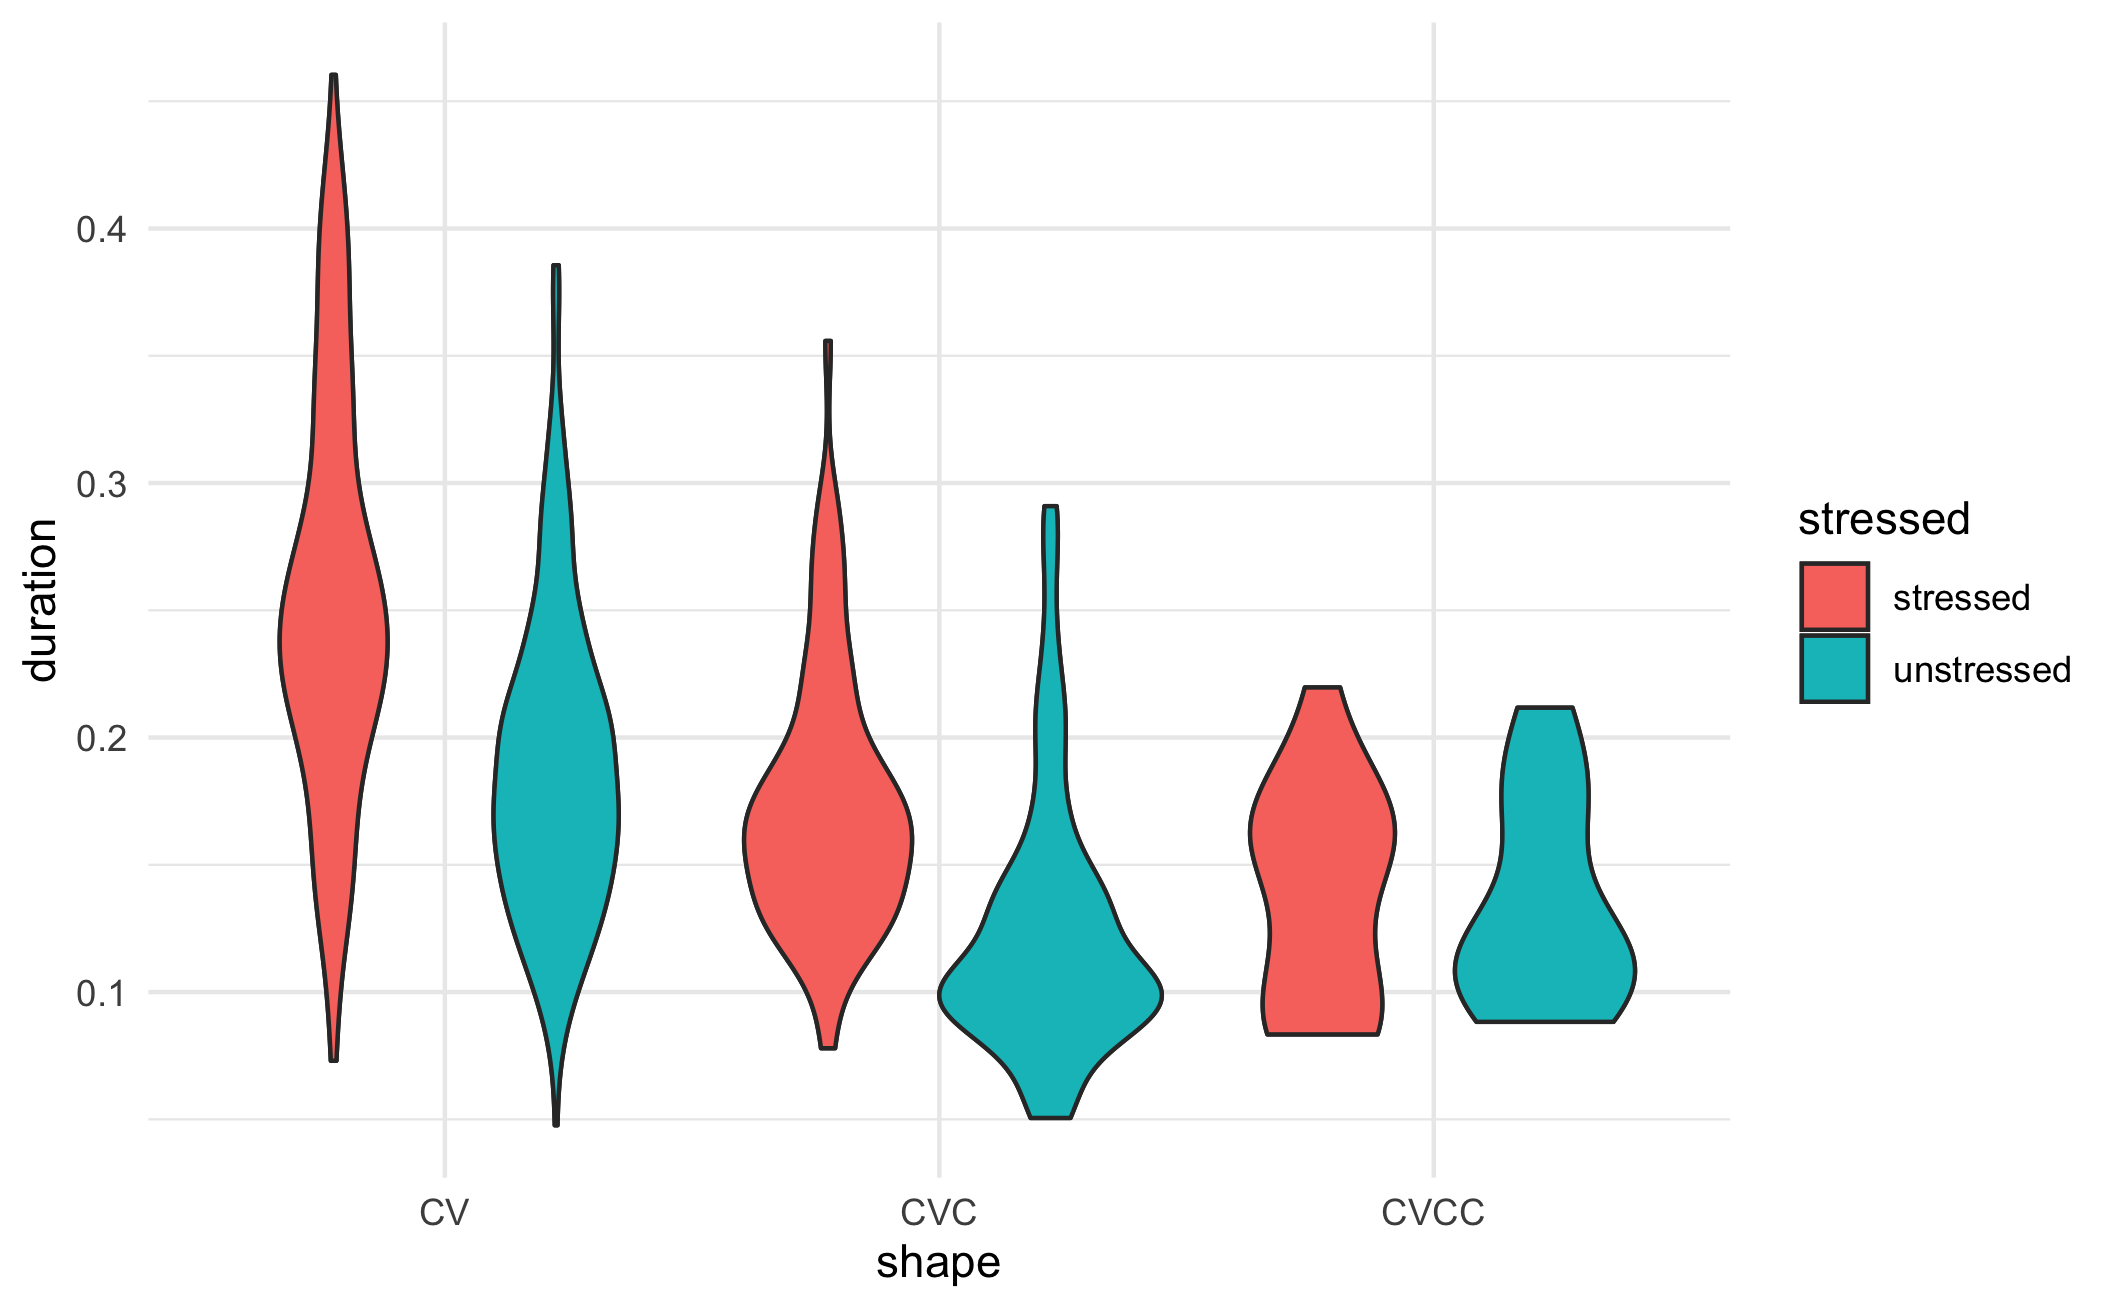
\includegraphics[width=\textwidth]{/Users/sarah/Git/regilaul_project/manuscript/results/dur_shapestress.png}
\caption{default}
\label{default}
\end{center}
\end{figure}



\begin{figure}[htbp]
\begin{center}
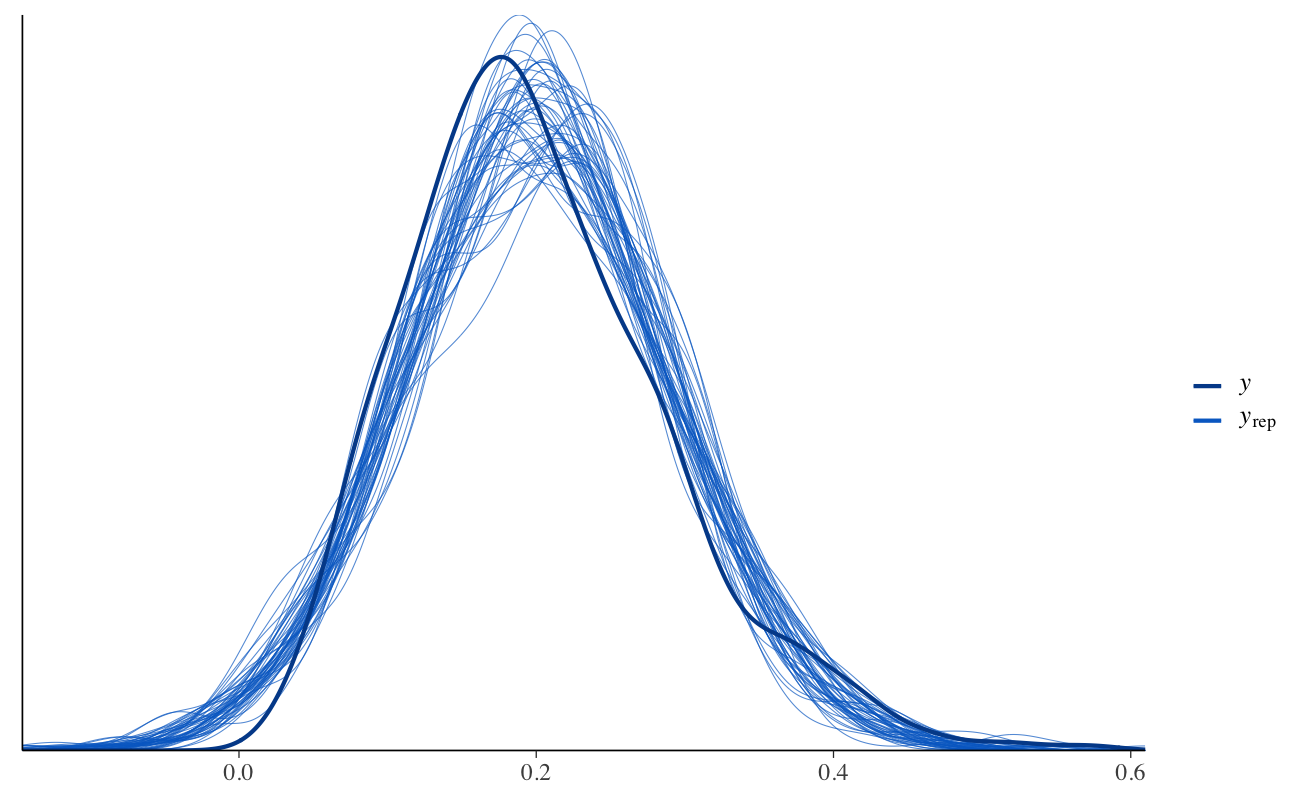
\includegraphics[width=\textwidth]{/Users/sarah/Git/regilaul_project/manuscript/results/figures/obs_samprep.png}
\caption{default}
\label{default}
\end{center}
\end{figure}

\begin{figure}[htbp]
\begin{center}
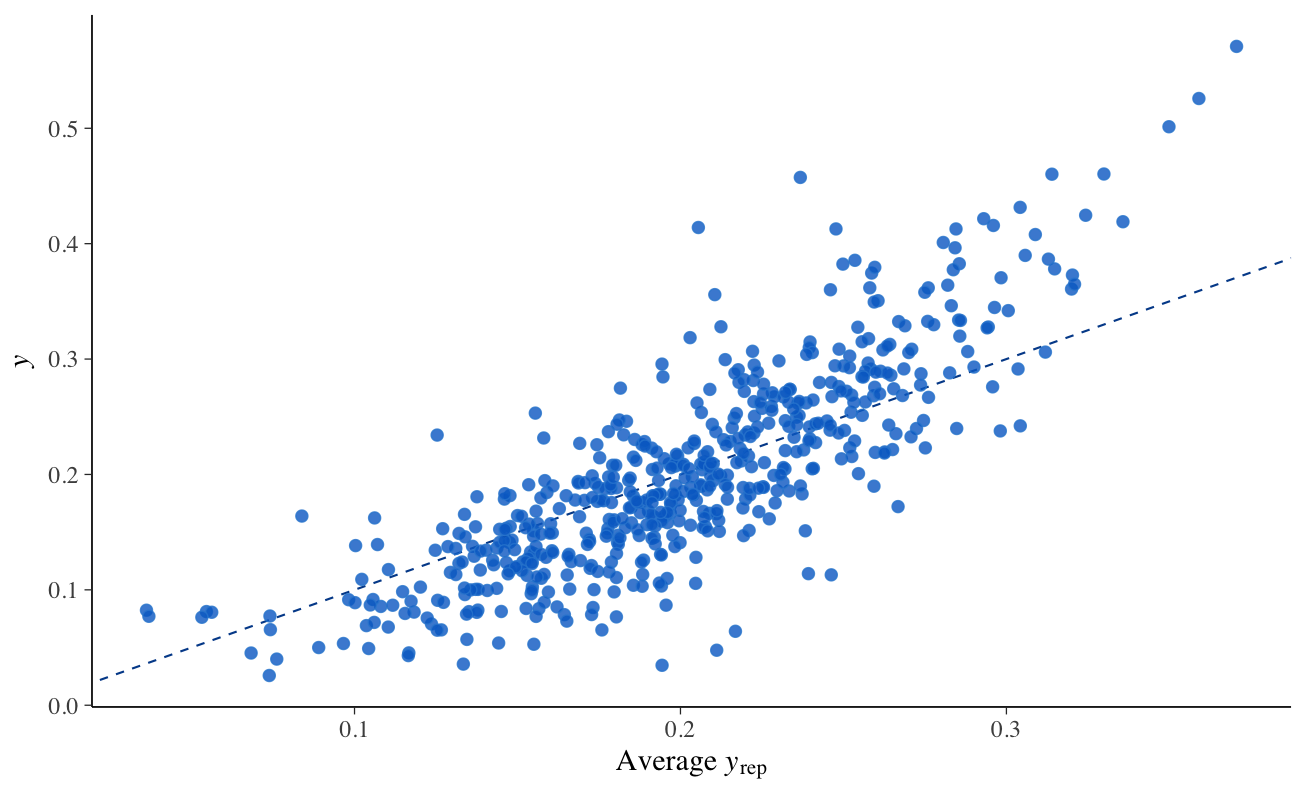
\includegraphics[width=\textwidth]{/Users/sarah/Git/regilaul_project/manuscript/results/figures/obs_sim.png}
\caption{default}
\label{default}
\end{center}
\end{figure}


%A similar trend is visible in  when the datum are grouped by subject: each performer utlilizes syllable nucleus lengthening in both song \ref{perfick} and word \ref{perfstr} positions of prominence. 


%
%\ref{density} shows violin density plots of vowel durations falling on and off the beat with stressed and unstressed syllables at the word level. Here each graph is one of the two quantities that occur in both stressed and unstressed positions in natural spoken Estonian. 
\subsection{Dispersion}
\begin{figure}[htb]
\begin{center}
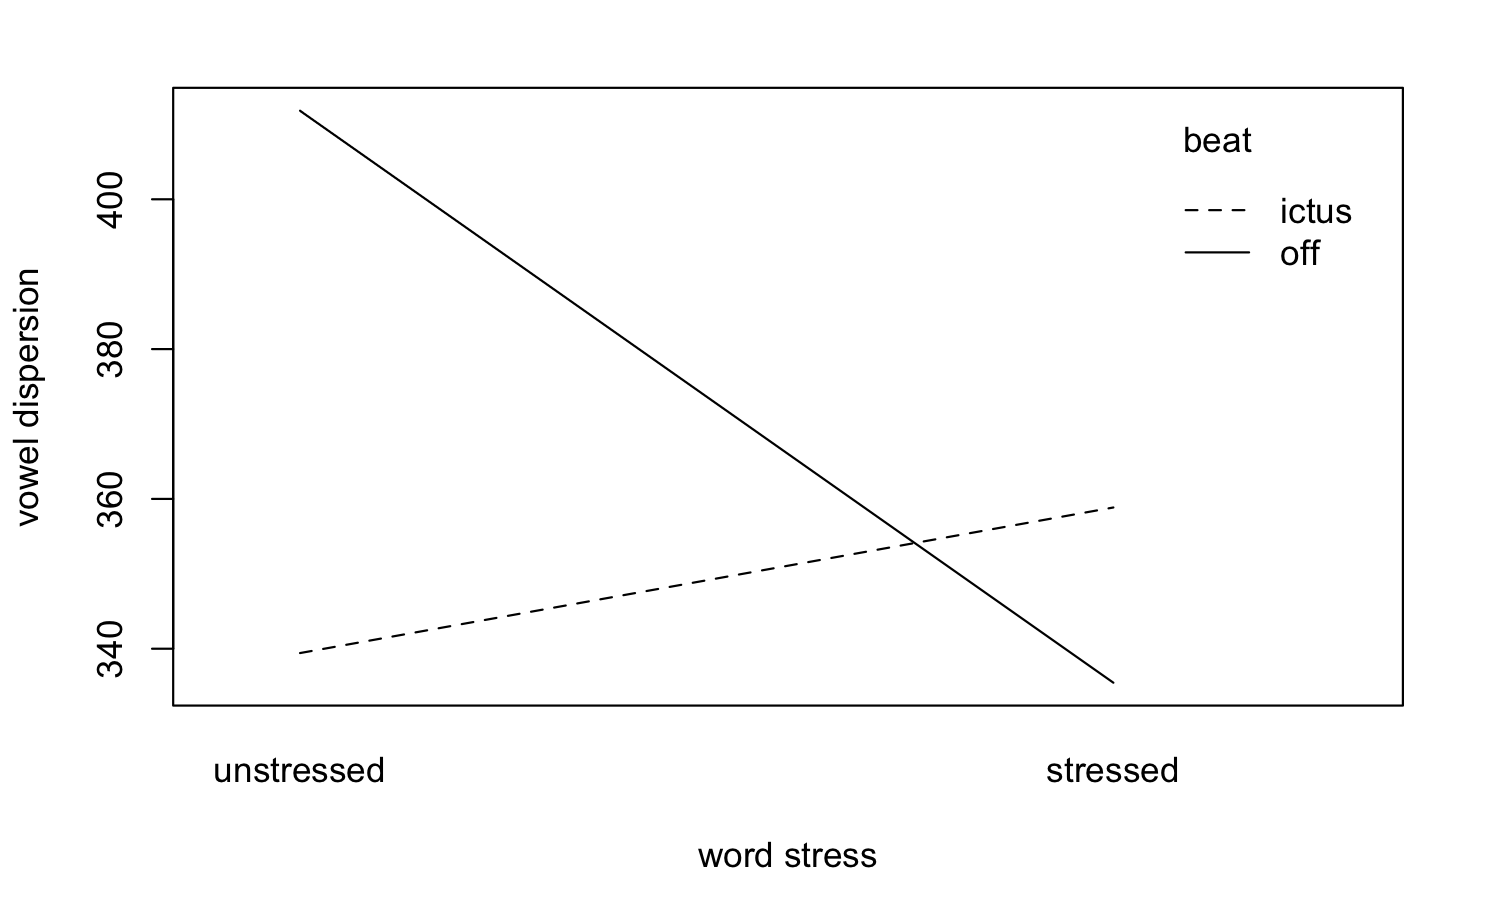
\includegraphics[width=\textwidth]{/Users/sarah/Git/regilaul_project/manuscript/results/figures/interact_space_strictus.png}


\caption{vowel dispersion interactions of word stress and beat position}
\label{density}
\end{center}
\end{figure}




%For each dependent measure, a linear model with all fixed and random effects was fitted using the statsmodels python library \citep{seabold2010statsmodels}. Exploratory analysis of data distribution confirmed normality of data and the residuals.
%Then, a linear model accounting for the potential interaction between stress and ictus is fitted, and a two-way anova is used to compare the two models. We reject the null hypothesis that the two models are of equal value, and continue with the larger nested model with interactions included (F = 6.17, {\it P} = 0.01). 

%Multi-factor ANOVA 





